\documentclass[report]{subfiles}
\begin{document}
\section{Wide Range Transconductance Amplifier}

\begin{figure}[htbp]
  \centering
  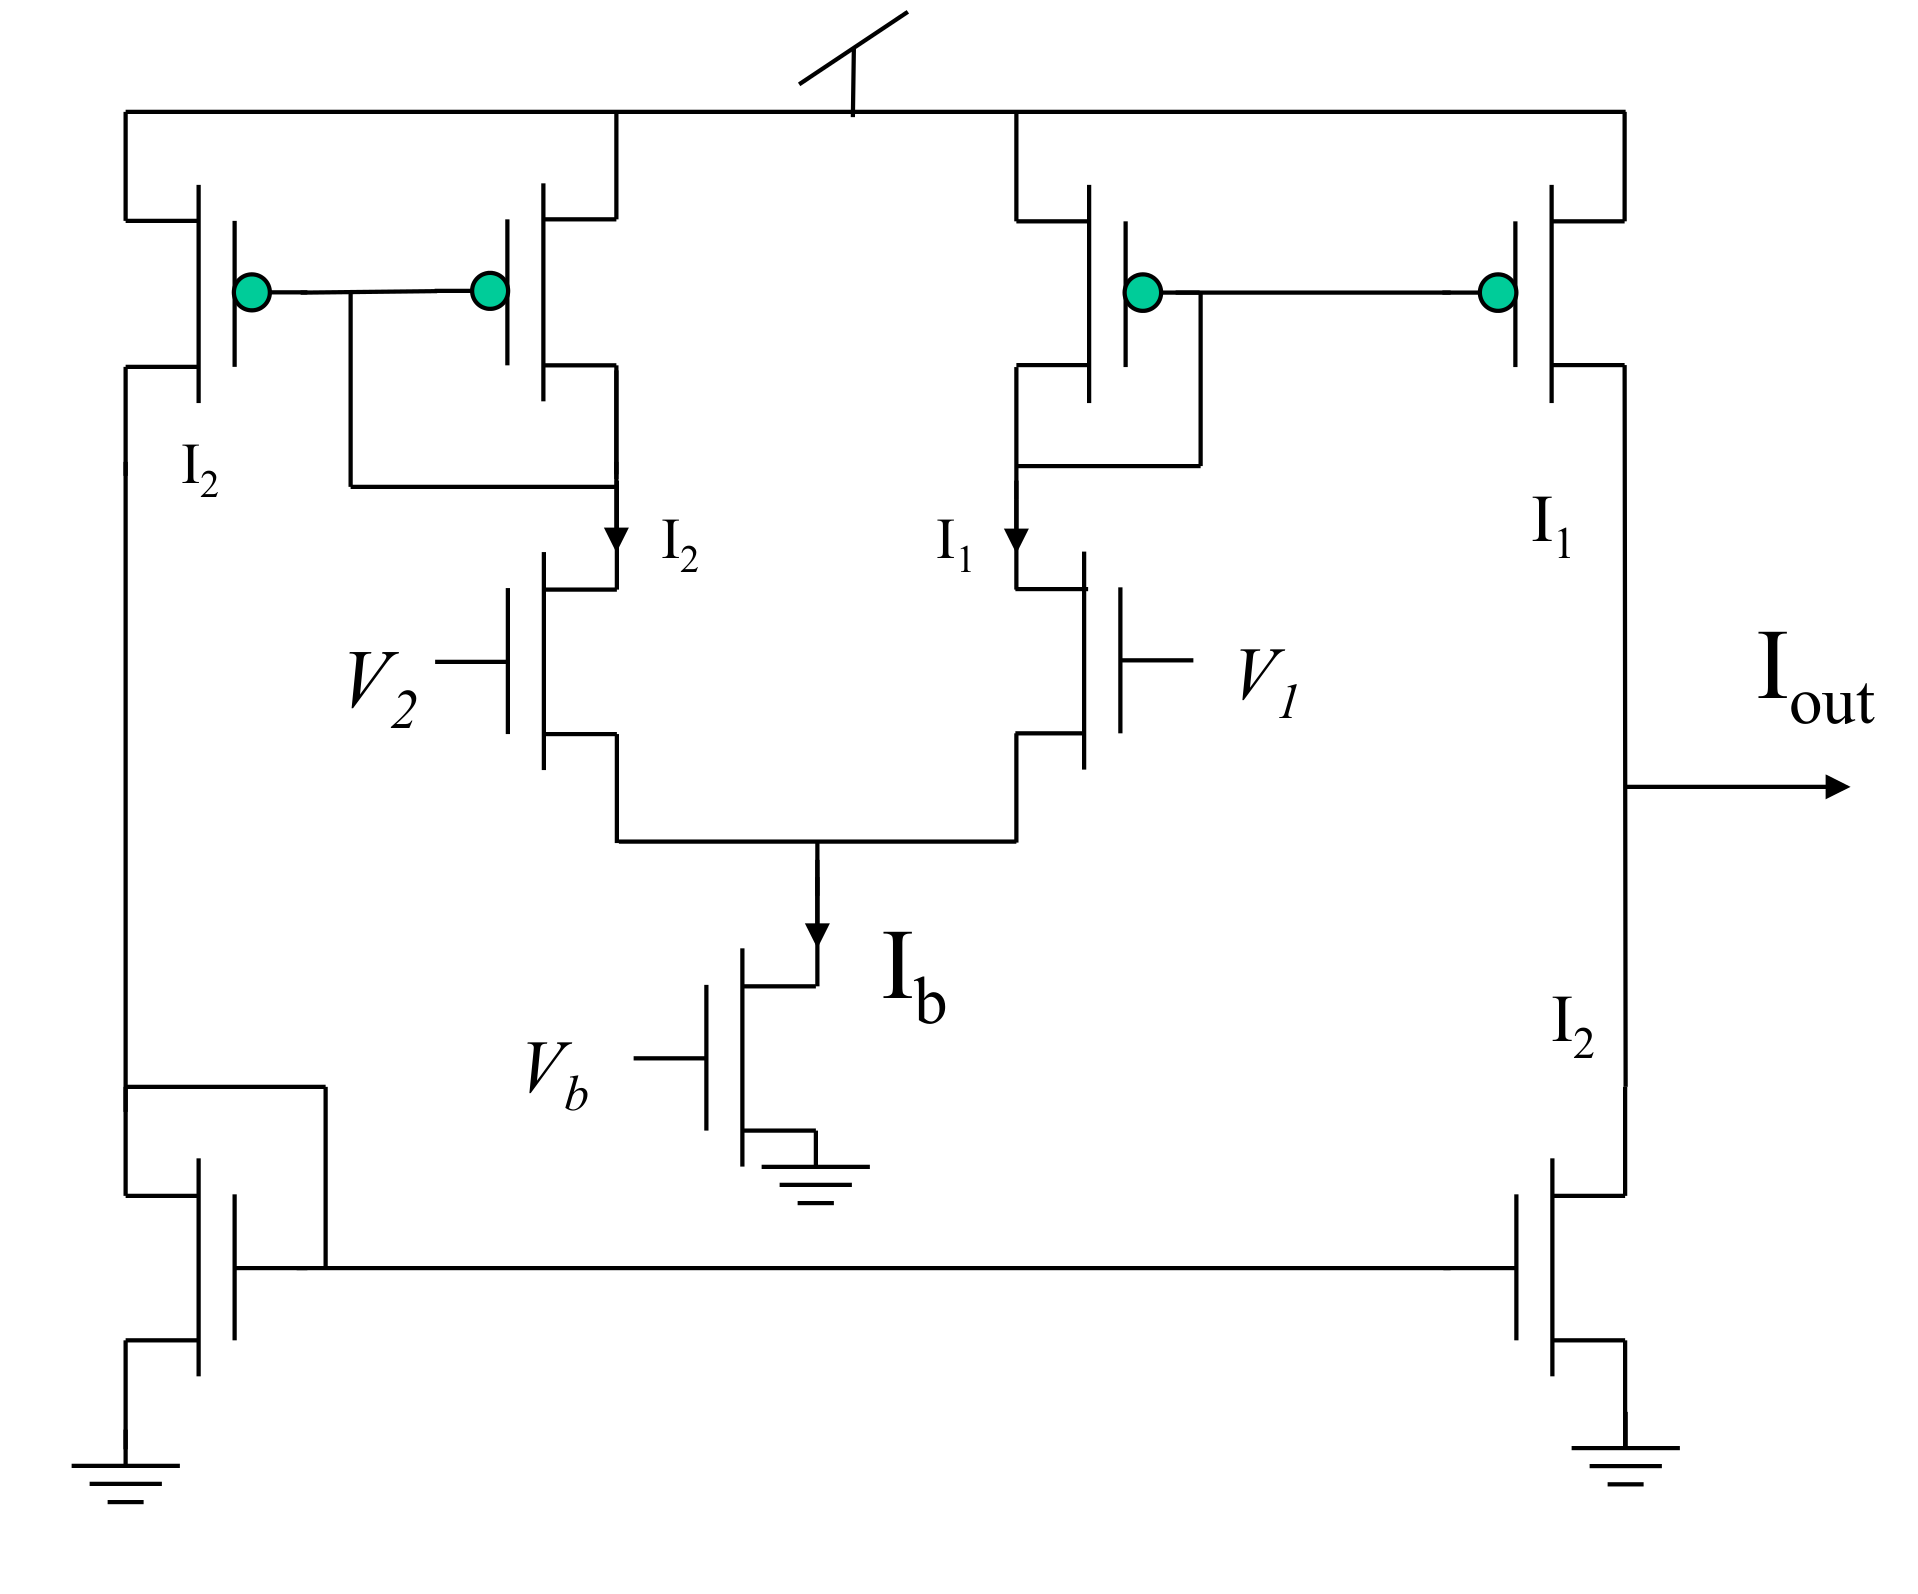
\includegraphics[scale=0.5]{pics/wide_range_transamp.png}
  \caption{Wide Range Transconductance Amplifier \cite{lec4}}
  \label{fig:wr_Transamp}
\end{figure}\bigskip


A wide-output range transconductance amplifier behaves very similar to a simple transconductance amplifier. Even though the circuit looks very complicated, it only consists of a differential pair and three current mirrors. The goal of these mirrors is to remove the restrictions on the output voltage of the amplifier.
\par Each branch of the differential pair is connected to a current mirror, but the currents $I_1$ and $I_2$ are still separated. After that, the same thing is done as in the simple transconductance amplifier, where one current (in Fig. \ref{fig:wr_Transamp} this would be $I_2$) is mirrored to the same node as the other one, and this node is connected to the output of the amplifier. The differential pair is now no longer connected to the output, which removes its restrictions from the allowed output condition. The new condition is
\( 4U_T < V_{out} < V_{dd} -4U_T\).
\end{document}